\subsection{Interactive Constrained MAP-Elites} \label{section:3}

The overarching goal of MI-CC is to collaborate with the user to produce content, either to optimize (i.e., exploit) their current design towards some goal or to foster (i.e., explore) their creativity by surprising them with diverse proposals. By implementing MAP-Elites~\citepsixth{p6Mouret2015} and continuous evolution into EDD, our algorithm can (1) account for the multiple dimensions that a user can be interested in, (2) explore multiple areas of the search space and produce a diverse amount of high-quality suggestions to the user, and (3) still evaluate how interesting and useful the tile distribution is within a specific room. Henceforth, we name the presented approach~\textbf{Interactive Constrained MAP-Elites} (IC MAP-Elites).

EDD uses a single-objective fitness function (shown in~\Cref{eq:fitness_func}) with a FI2Pop genetic algorithm, where fitness is a weighted sum divided equally between (1) the inventorial aspect of the rooms and (2) the spatial distribution of the design. $f_{inventorial}$ is the evaluation of the aggregated and normalized quality of treasures, enemies, and doors (inventorial patterns). $f_{spatial}$ refers to the quality and distribution of chambers, i.e. open areas in the room and corridors (both categorized as spatial patterns), and the meso-patterns that are created within chambers and their quality. Quality refers to the positioning, safety, composition, and relation between patterns. The fitness adapts to the user's current design, automatically informing target ratios and distributions to be used as targets. In-depth evaluation of EDD's fitness function, as well as discussion and explanation of the quality of each inventorial, spatial, and meso pattern, can be found in~\citepsixth{p6Alvarez2018a,p6Baldwin2017,p6Baldwin2017a}.

% . An in-depth explanation and formulas of EDD's fitness function can be found in~\citepsixth{p6Alvarez2018a, Baldwin2017}Where $f_{inventorial}$ is the evaluation of the aggregated and normalized quality of treasures, enemies, and doors (inventorial patterns). Quality refers to positioning, safety, and the relation between inventorial patterns. $f_{spacial}$ refers to the quality and distribution of chambers i.e. open areas in the room, and corridors, and the meso-patterns that are created within chambers and their quality. 

% , which relates to the placement of enemies and treasures in relation to doors and target ratios, and (2) the spatial distribution of the design patterns, which refers to the distribution between corridors and rooms, and the meso-patterns that those encompass. The fitness is shown in~\Cref{eq:fitness_func}, where 

\begin{equation} 
\label{eq:fitness_func}
f_{fitness}(r) = \frac{1}{2}f_{inventorial}(r) \,+ \, \frac{1}{2}f_{spatial}(r)
\end{equation}

%EDD uses a single-objective fitness function with a FI2Pop genetic algorithm, which adapts to the user's current design. Fitness is a weighted sum divided equally between (1) the inventorial aspect of the rooms, which relates to the placement of enemies and treasures in relation to doors and target ratios, and (2) the spatial distribution of the design patterns, which relates to the distribution between corridors and rooms, and the meso-patterns that those encompass. Target ratios and distributions are automatically based on the user's design. An in-depth explanation of EDD's fitness function can be found in~\citepsixth{p6Alvarez2018a, Baldwin2017}.

%In addition, 
% The overarching goal of MI-CC is to collaborate with the user to produce content, either to optimize (i.e. exploit) their current design towards some goal or to foster (i.e. explore) their creativity by surprising them with diverse proposals. By implementing MAP-Elites~\citepsixth{p6Mouret2015} and continuous evolution into EDD, our algorithm can (1) account for the multitude of dimensions that a user can be interested in, (2) explore multiple areas of the search space and produce a diverse amount of high-quality suggestions to the user, and (3) still evaluate how interesting and useful the tile distribution is within a specific room. Henceforth, we name the presented approach \textbf{Interactive Constrained MAP-Elites} (IC MAP-Elites).

% ince EDD already uses a FI2Pop, we took the Constrained MAP-Elites, presented by Khalifa et al.~\citepsixth{p6Khalifa2018}, as a starting point. The illuminating capabilities of MAP-Elites explore the search space with the constraints aspects of FI2Pop. This approach manages two different populations, a feasible and an infeasible one, within each cell. Individuals move across cells when their dimension values change, or between the feasible and infeasible population according to their fulfillment of the feasibility constraint.

Furthermore, IC MAP-Elites adds interactive and continuous evolution to the Constrained MAP-Elites presented by Khalifa et al.~\citepsixth{p6Khalifa2018}. This is done through an adaptive fitness function (based on the designer's design) that adapts the content generation, and by enabling the designer to flexibly change the feature dimensions and the granularity of the cells. It also adapts the usability of MAP-Elites to generate dungeon and adventure levels in an MI-CC system, which gives more control to the designers over non-intuitive parameters and aspects of MAP-Elites, while providing a richer set of high-performing and diverse suggestions.

% Furthermore, IC MAP-Elites adds interactive evolution to the Constrained MAP-Elites presented by Khalifa et al.~\citepsixth{p6Khalifa2018}, adapts the usability of MAP-Elites in an MI-CC system, which gives more control to the designers over non-intuitive parameters and aspects of MAP-Elites, adds continuous evolution by adapting the generation to the designer's design over time, and explores the usability of IC MAP-Elites to generate dungeon and adventure levels.

% , and through this in depth evaluation, we assess its feasibility and adaptability to create dungeons and adventure levels. Through the in-depth evaluation 

% Specifically, IC MAP-Elites have the following novel characteristics: 
% % Here is where I should bring what are the differences with Constrained MAP-Elites

% \begin{itemize}
%     % \item Adapting~\acrshort{mape} to be used to co-design levels by proposing suggestions in an~\acrshort{micc} system.
%     \item MAP-Elites adapted to be used in a MI-CC system to collaborate and interact with the designer.
%     \item Use of MAP-Elites to create dungeons and adventure levels.
%     \item Continuously adapting the fitness landscape and search space based on the designer's creation, which in turn, makes MAP-Elites continuously adapting to a changing space.
%     \item Customizable behavioral feature dimensions as part of the designer's ability to interact with the system. By changing the feature dimensions, pressure is imposed in the algorithm to adapt the search as the behavior dimensions are no longer the same (i.e., the niches changed).
% \end{itemize}

% In terms of the~\acrshort{ea} components, our implementation of~\acrshort{icmape} in~\acrshort{edd} uses direct encoding similar to the one depicted in figure~\ref{fig:directENCOD}, selection is through competition of individuals in each cell population, and selected individuals are applied crossover and mutation. Finally, the replacement strategy is elitist; if any offspring is better than individuals in their cell, these are replaced. 

\subsubsection{Illuminating Dungeon Populations with MAP-Elites}

MAP-Elites explores the search space more vastly by separating interesting feature dimensions, that affect different aspects of the room, such as playability or visual aesthetics, from the fitness function, to categorize rooms into cells. %as intrinsic measures of rooms to categorize them into niches (cells). %With such niches, we are able to present diverse suggestions to the user while still maintaining a high quality on them.

In this subsection, we firstly present all the current feature dimensions identified and implemented in EDD, secondly, we explain the transition from fixed evolution to continuous evolution, and lastly, we introduce and outline the IC MAP-Elites algorithm.

\paragraph{Dimensions}\label{sec:dimensions}
%
Dimensions in MAP-Elites are identified as those aspects of the individuals that can be calculated in the behavioral space, and that are independent of the fitness calculation. These are crucial in MAP-Elites, as they represent the discretized dimensions where individuals will be retained as the space is explored. %intrinsic, and more important, independent from the fitness calculation. %, although, as we present in section \Cref{section:results}, the occurrence of individuals in certain dimensional cells correlates with lower or higher fitness scores. 
EDD offers the designer the possibility to choose among the following dimensions, two at a time (examples of rooms generated using the dimensions are shown in~\Cref{figs:dimensions-example}):
%Currently, we use five different dimensions: (1) symmetry and (2) similarity, related to visual aesthetics, (3) number of meso-patterns and (4) spatial-patterns, related to the presence of patterns in the room, and used to exploit the design pattern characteristics of the room, and (5) linearity, linked to the type of gameplay and possibilities in the room. The user can only choose a pair of dimensions at a time, since presenting higher dimensions would be undesirable and non-understandable for the user. 

\textbf{Symmetry (Sym) and Similarity (Sim).} We choose Symmetry as a consideration of the aesthetic aspects of the edited room since symmetric structures tend to be more visually pleasing for the user and relate to fairness distribution and human-made structures~\citepsixth{p6marinho2016-symmetry,p6Alvarez2018a,p6Liapis2012-adaptiveVisual}. Similarity is used to present the user variations of their design but still preserving their aesthetical edits. Symmetry is assessed using only impassable tiles (i.e., walls) and evaluated along the X and Y axes and diagonals. The highest value is normalized by the total amount of walls and used as the symmetry score (\Cref{eq:Symmetry}). Similarity is calculated by comparing tile by tile with the target room (\Cref{eq:similarity}). In-depth descriptions and evaluations can be found in~\citepsixth{p6Alvarez2018a}, where both dimensions were used as aesthetic fitness evaluations.

% Symmetry is evaluated along the X and Y axes, backslash, and front slash diagonal, and the highest value  is used as to how symmetric a room is. 

% Formulas, information, and support for both evaluations are explained in greater detail in~\citepsixth{p6Alvarez2018a}, where both of them were used as aesthetic fitness evaluations.

\begin{equation} \label{eq:Symmetry}
D_{sym} = \frac{highestSymmetricValue} {totalWalls}
\end{equation}

\begin{equation} \label{eq:similarity}
D_{sim} = \frac{totalTiles - notSimilarTiles} {totalTiles}
\end{equation}

\textbf{Number of Meso-patterns (NMP).} The number of meso-patterns correlates to the type and amount of encounters the designer wants the user to have in the room in a more structured manner. The considered patterns are the treasure room (tr), guard rooms (gr), and ambushes (amb). Meso-patterns associate utility to a set of tiles in the room, for instance, a long chamber filled with enemies and treasures could be divided into 2 chambers, the first one with enemies and the second one with treasures so the risk-reward encounter is more understandable for the player. Since we already analyze the rooms for all possible patterns, the number of meso-patterns is simply $\#MesoPat=tr, gr, amb \in AllPatterns$. \Cref{eq:meso-pat-eq} presents the dimensional value, and since the used meso-patterns can only exist in a chamber, we normalize by the maximum amount of chambers in a room, which are of a minimum size of $3\times3$, and results in $Max_{chambers}=\left\lfloor Cols/3 \right\rfloor \cdot \left\lfloor Rows/3 \right\rfloor$.

%All variables will be defined, and such variables names will  be replaced

%\begin{equation} \label{eq:meso-pat-eq}
%D_{mesoPat} = \min{ \left\{     \dfrac{\#MesoPat}{Max_{chambers}}, 1.0}
%\right\} }
%\end{equation}

\begin{equation} \label{eq:meso-pat-eq}
D_{NMP} = \min \left\{ \dfrac{\#MesoPat}{Max_{chambers}}, 1.0 \right\}
\end{equation}


\textbf{Number of Spatial-patterns (NSP).} By spatial-patterns we mean chambers (c), corridors (cor), connectors (con), and nothing (n). We identify the number of spatial-pattern relates to how individual tiles group (or not) together to form spatial structures in the room. The higher the amount of spatial-patterns the lesser tiles will be group together in favor of more individualism. For instance, a room with one spatial-pattern can be one with no walls and just an open chamber, while a room with a higher number of spatial-patterns would subdivide the space with walls, using tiles for more specific patterns. \Cref{eq:spatial-pat-eq} presents how we calculate the value for such a dimension. The number of spatial patterns is simply $\#SpatialPat=c, n, cor, con \in AllPatterns$, we then normalize it by the largest side of the room and multiply it by a constant value, determined as $K=4.0$ through a process of experimentation.% since it resulted in a good estimation of the amount of spatial patterns in the room.

%\textit{not sure of this example} For instance, depicted in figure XXX a., a chamber is a micro-pattern that associate several tiles to one specific pattern, if we then simply add a wall in the middle of it as in figure XXX b., we break the pattern into many other patterns that in turn, create a different type of challenge for the user, a loop. We finally calculate the dimension value with the following formula:

%\begin{equation} 
%\label{eq:spatial-pat-eq}
%D_{spatialPat} = 
%\min{ \left\{ 
%    \frac{\#SpatialPat}{\max\left\{{Cols, Rows}\right\} * \textit{K}}, 1.0}
%\right\}
%\end{equation}

%\begin{equation} 
%\label{eq:spatial-pat-eq2}
%D_{spatialPat} = 
%\min{ \left\{ 
%    \frac{\#SpatialPat}{\max\left\{{Cols, Rows}\right\} * \textit{K}}, 1.0}\right\} }
%\end{equation}

\begin{equation} 
\label{eq:spatial-pat-eq}
D_{NSP} = \min\left\{\frac{\#SpatialPat}{\max\left\{{Cols, Rows}\right\} \cdot \textit{K}}, 1.0\right\}
\end{equation}

\textbf{Linearity (Lin).} Linearity represents the number of paths that exist between the doors in the room. This relates to the type of gameplay the designer would like the room to have by the distributions of walls among the room. Having high linearity in a room does not need to only be by having a narrow corridor between doors but could also be generated by having all doors in the same open space (i.e. the user would not need to traverse other areas) or by simply disconnecting all paths between doors. \Cref{eq:Linearity-eq} shows the linearity calculation. Due to the use of patterns, we calculate the paths between doors as the number of paths that exist from a spatial-pattern containing a door to another. Finally, this is normalized by the number of spatial patterns in combination with the number of doors and their possible neighbors.

\begin{equation} \label{eq:Linearity-eq}
D_{lin} = 1 \text{--} \frac{AllPathsBetweenDoors} {\#spatialPat + \#NeighborsPerDoor}
\end{equation}

%Work in progress

\textbf{Inner Similarity (IS).} Inner similarity compares the target room to one generated, considering only the distribution and ratios of micro-patterns in both rooms rather than any aesthetic criteria. Specifically, we look into the density ($den$) and sparsity ($spa$) of enemies ($en$), treasures ($tre$), and walls ($wal$) in the target room ($R_{tg}$) in comparison with the generated rooms ($R_{gen}$). To calculate the density and sparsity of each micro-pattern, we first clustered all micro-patterns of the same kind based on the distance within the room (i.e. $distance=1$). We then use these clusters to calculate the density (\Cref{eq:dens}) using as density threshold $\theta=4$ for treasures and enemies, and $\theta=6$ for walls, and calculate the sparsity (\Cref{eq:spars}). Finally, we calculate the difference between each distribution in $R_{tg}$ and $R_{gen}$, linearly combining all the values into the IS measure as in \Cref{eq:innersimDim}.

\begin{equation} \label{eq:dens}
den(x)= \dfrac{\sum_{i=1}^{\left | clusts \right |}\min \left\{1.0, \dfrac{\left | clust_{i} \right |}{\theta_{x}}\right\}}{\left | clusts \right |}
\end{equation}

\begin{equation} \label{eq:spars}
spa(x)= \dfrac{\sum_{i=1}^{\left | clusts \right |}\sum_{j=1, j\neq i}^{\left | clusts \right |}\dfrac{Dist(clust_{i}, clust_{j})}{\left | room \right |}}{\left | clusts \right | \cdot (\left | clusts \right | - 1)}
\end{equation}

\begin{equation} \label{eq:innersimDim}
\begin{split}
D_{IS} = \sum_{i=1}^{micropats}\left | den(R_{gen}) - den(R_{tg}) \right | + \\ \left | spa(R_{gen}) - spa(R_{tg}) \right |
\end{split}
\end{equation}

\textbf{Leniency (Len).} Leniency calculates how challenging a room is at any given point. It is based on the amount of enemies and treasures that are in a room, their density and sparsity calculated as in eq. (\ref{eq:dens}) and (\ref{eq:spars}), respectively, and how safe the doors are (i.e. entry/exit points) calculated as in ~\citepsixth{p6Baldwin2017}. We base our calculation in the idea that rooms are less lenient the more enemies they contain as well as how they are distributed, counterbalanced by the number of treasures as they reward players. We calculate the dimension value for each room as shown in (\Cref{eq:lendim}), which uses a combination of precomputed non lenient (\Cref{eq:nonlenvals}) and lenient (\Cref{eq:lenvals}) values.


\begin{equation} \label{eq:nonlenvals}
\begin{split}
nonLenientValues = w_{0} \cdot \log_{10}(\left | en \right | \cdot spa(en)) + \\ w_{1} \cdot \log_{10}(\left | en \right | \cdot den(en)) + w_{2} \cdot (1.0 - door_{safety})
\end{split}
\end{equation}

\begin{equation} \label{eq:lenvals}
\begin{split}
LenientValues = \sfrac{1}{2} \log_{10}(\left | tre \right | \cdot spa(tre)) + \\ \sfrac{1}{2} \log_{10}(\left | tre \right | \cdot den(tre))
\end{split}
\end{equation}

\begin{equation} \label{eq:lendim}
D_{len} = 1.0 - (nonLenientValues - (\sfrac{1}{2} \cdot LenientValues))
\end{equation}

% \begin{figure}[h]
% \centerline{\includegraphics[width=9cm]{figures/target-rooms-figure.png}}
% \caption{Target Rooms used in the experiments.}
% \label{figs:targetRooms}
% \end{figure}

% \begin{figure}[h]
% \centerline{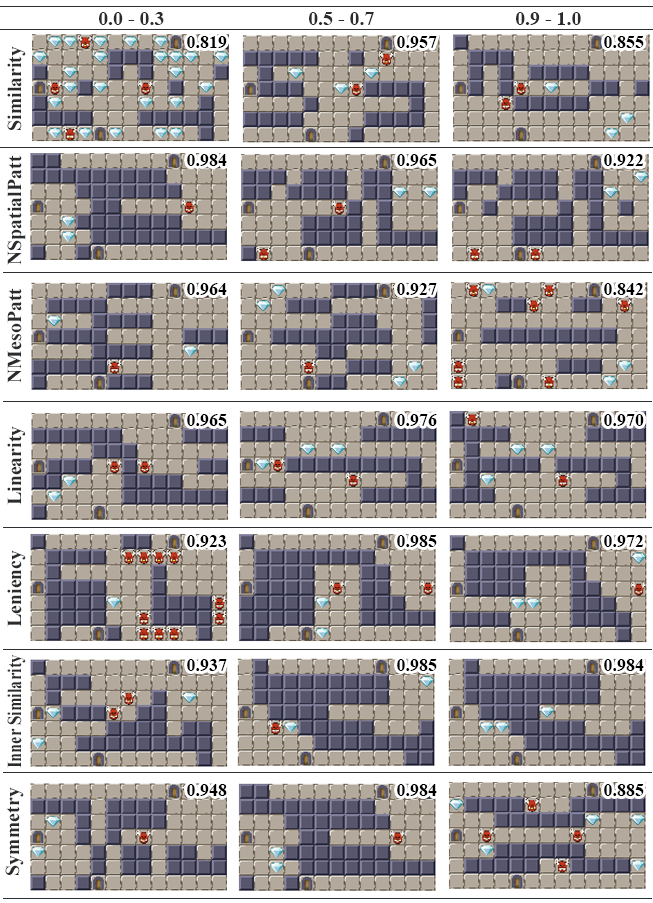
\includegraphics[width=9cm]{figures/figure-all-dimensions-final.png}}
% \caption{Example of Elites generated using IC MAP-Elites. Each row represents an independent run of the algorithm using the dimension specified to the left and \Cref{figs:targetRooms}.b as target room. each column splits the dimension score into three intervals: 0.0-0.3 (low), 0.5-0.7 (medium), and 0.9-1.0 (high). Each cell displays (top-right) the fitness of the optimal individual in its related interval.% used of of each dimension (each row)%Shouldn't be work in progress now %Figure is work in progress (among other things, it is missing the fitness of each of the generated rooms + the "dimension values" of the edited room) to present each what the EA generates based on the different dimensions using room (a) as target - so it is clear for the reader how each dimension looks and to discuss more in detail
% }
% \label{figs:dimensions-example}
% \end{figure}

\begin{figure}[h]
\centering
     \subfloat[Basic room\label{figs:targetRoomsBas}]{%
       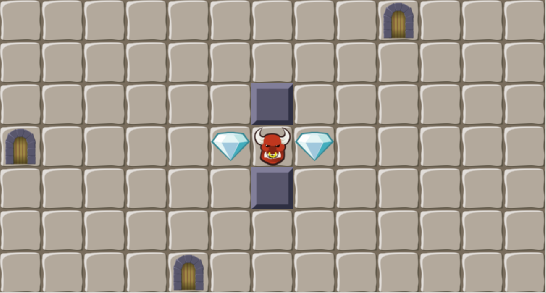
\includegraphics[width=0.23\textwidth]{figures/figure2a.png}
     }
    %  \centerhfill
     \subfloat[Complex room\label{figs:targetRoomsComp}]{%
       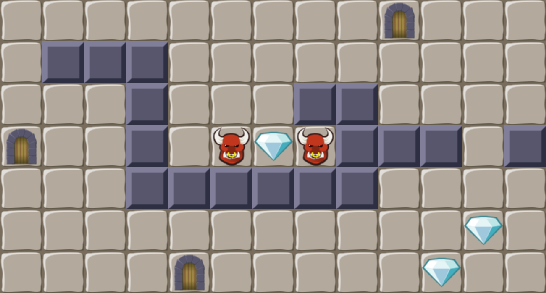
\includegraphics[width=0.23\textwidth]{figures/figure2b.png}
     }\hfill
     \subfloat[Example Elites generated using IC MAP-Elites with (b) as target. \label{figs:dimensions-example}]{%
       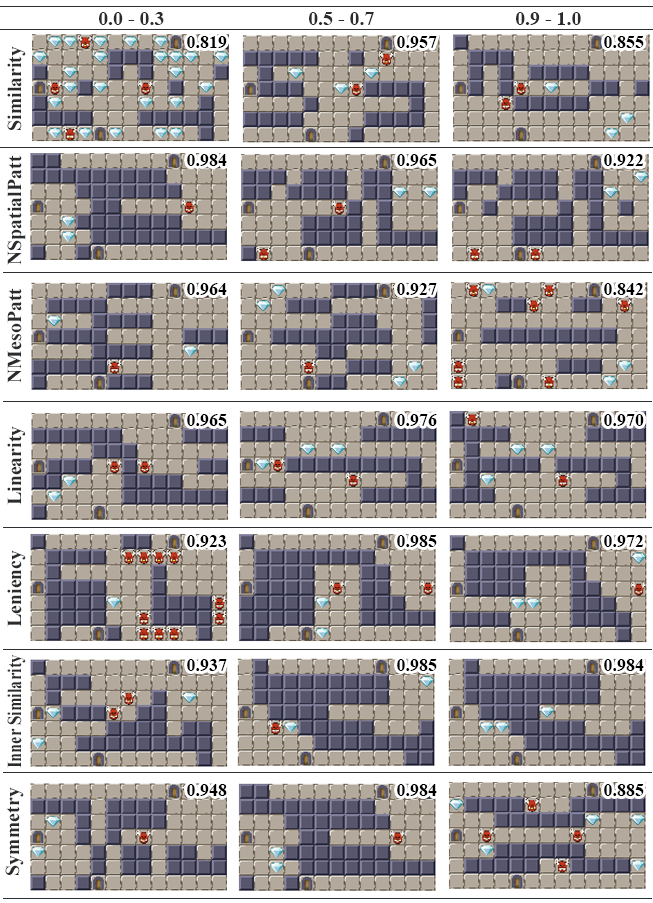
\includegraphics[width=0.45\textwidth]{figures/figure2c.png}
     }\hfill

% \centerline{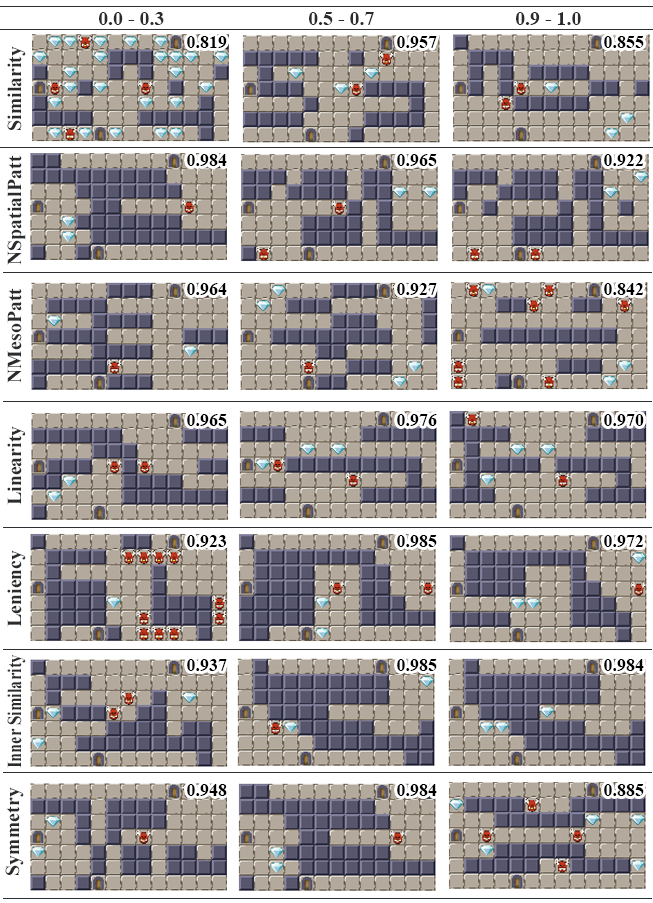
\includegraphics[width=9cm]{figures/figure-all-dimensions-final.png}}
\caption{(a) and (b) represent target rooms used in the experiments. Each row in (c) represents an independent run of the algorithm using the dimension specified to the left. Each column splits the dimension score into three intervals. Each cell displays (top-right) the fitness of the optimal individual in its related interval.% used of of each dimension (each row)%Shouldn't be work in progress now %Figure is work in progress (among other things, it is missing the fitness of each of the generated rooms + the "dimension values" of the edited room) to present each what the EA generates based on the different dimensions using room (a) as target - so it is clear for the reader how each dimension looks and to discuss more in detail
% (a) and (b) represent target rooms used in the experiments. (b) is a more developed room with meso patterns. Each row in (c) represents an independent run of the algorithm using the dimension specified to the left. Each column splits the dimension score into three intervals: 0.0-0.3 (low), 0.5-0.7 (medium), and 0.9-1.0 (high). Each cell displays (top-right) the fitness of the optimal individual in its related interval.
}
\end{figure}

\paragraph{Continuous and Interactive Evolution}

%Creation tools are highly dynamic, the user might have an empty canvas in one moment, and after a few interactions over the course of some seconds, they might have a complex room with multiple paths and challenges for the user, and even more ideas on what to do next. Thus, the nature of the tool and the fast-paced interactions require a dynamic and continuous EA that can cope with the requirements of the user and adapt seamlessly to the new changes.

%This interesting paradigm shift, allows the user to focus solely in the design of the rooms while in the background, the EA is adapting to those new designs, rather than waiting for the EA to present suggestions.

Since EDD already uses a FI2Pop, we took the Constrained MAP-Elites, presented by Khalifa et al.~\citepsixth{p6Khalifa2018}, as a starting point. The illuminating capabilities of MAP-Elites explore the search space with the constraints aspects of FI2Pop. This approach manages two different populations, a feasible and an infeasible one, within each cell. Individuals move across cells when their dimension values change, or between the feasible and infeasible population according to their fulfillment of the feasibility constraint.

As discussed by Takagi, interactive evolution is a way to improve the capabilities of Evolutionary Algorithms (EA) by having humans in-the-loop to subjectively evaluate individuals. This hybrid approach has proven to reach better and more adaptive results but at the expenses of user's fatigue and user's understanding of the EA and the given problem~\citepsixth{p6Takagi2001-InteractiveEvo}. However, in EDD and the IC MAP-Elites, the user does not directly evaluate individuals; instead, IC MAP-Elites adapts the fitness and search based on different interactions the designer has with the algorithm. 

The designer can interact with the crossover step by locking tiles~\citepsixth{p6Alvarez2018a}, and with the dimensions and cells by changing the dimensions and granularity for the MAP-Elites, enabling IC MAP-Elites to focus on different regions of the generative space. Furthermore, IC MAP-Elites constantly updates the target room and configuration with the most recent version of the designer's design. Once the suggestions are broadcasted, that room is incorporated without changes to the population of individuals in the corresponding cell.

This adaptability feature and different designer's indirect interactions with IC MAP-Elites, enables the implementation of continuous and interactive evolution, as well as allowing the designer to focus solely in the design of the room, while IC MAP-Elites adapts to the new designs.



%EDD implements continuous evolution in two ways. First, the EA constantly updates the target room and configuration with the most recent version of the user’s design, and once the suggestions are broadcasted, that room is incorporated without changes to the population of individuals in the corresponding cell. Secondly, by changing the dimension information and their granularity for the MAP-Elites, which can be done at any given time by the designer. 
%&in which case, the EA recalculates the cells with the new dimensions and assign the population to the correct cell.% would reset all the cells, calculate their new dimension values and assign the previous populations to the correct cell.


\algblockdefx{MRepeat}{EndRepeat}{\textbf{repeat}}{}
\algnotext{EndRepeat}

\begin{algorithm}
%\algsetup{linenosize=\tiny}
\footnotesize
\caption{Interactive Constrained MAP-Elites}\label{alg:IC-MAPE}
\begin{algorithmic}[1]
\Procedure{IC MAP-Elites($\protect[\{d_1,v_1\},...,\{d_n,v_n\}]$)}{}
\State $target \gets curEditRoom$ \Comment{Always in background}
\State createCells$(\protect[\{d_1,v_1\},...,\{d_n,v_n\}])$
\For{$i \gets 1$ to $PopSize$} %\Comment{$PopSize \gets 1000$}
     \State add mutate$(target)$ to $population$
\EndFor
\State CheckAndAssignToCell$(population)$ 
\While {true} \Comment{start continouous evo}
    \For{$generation \gets 1$ to $publishGen$}
        \If {$\textit{dimensionsChanged}$}
            \State $previousPop \gets cells_{pop}$
            \State createCells$(newDimensions)$
            \State checkAndAssignToCell$(previousPop)$ 
        \EndIf
        \MRepeat{ \text{[for feasible \& infeasible pop.]}}
            \For{$i \gets 1$ to $ParentIteration$}
                \State $curCell \gets \text{rndCell}(cells)$
                \State add tournament$(curCell)$ to $parent$
            \EndFor
            \State $offspring \gets  \text{crossover}(Parent)$
            \State checkAndAssignToCell$(offspring)$
        \EndRepeat
        \State sortAndTrim$(cells)$
    \EndFor
    \State broadcastElites() \Comment{render elites}
    \State $pop' \gets cells_{population}$
    \State add mutate$(cells_{pop})$ to $pop'$
    \State add $target$ to $pop'$
    \State checkAndAssignToCell $(pop')$
    \State sortAndTrim$(cells)$
\EndWhile
\EndProcedure
\Procedure{createCells(dimensions)}{}
    \ForEach{$dim \in dimensions $}
        \State add newCell$(dim_d, dim_v)$ to $cells$
    \EndFor
\EndProcedure
\Procedure{$\protect \text{check\&AssignToCell}(curPopulation)$}{}
    \ForEach{$individual \in curPopulation $}
        \State $individual_f \gets evaluate(individual)$ 
        \State $individual_d \gets dim(individual)$
        \State add $individual$ to $cell_{pop}(individual_d)$
    \EndFor
\EndProcedure
\end{algorithmic}
\end{algorithm}

% \begin{figure*}[h]
% \centerline{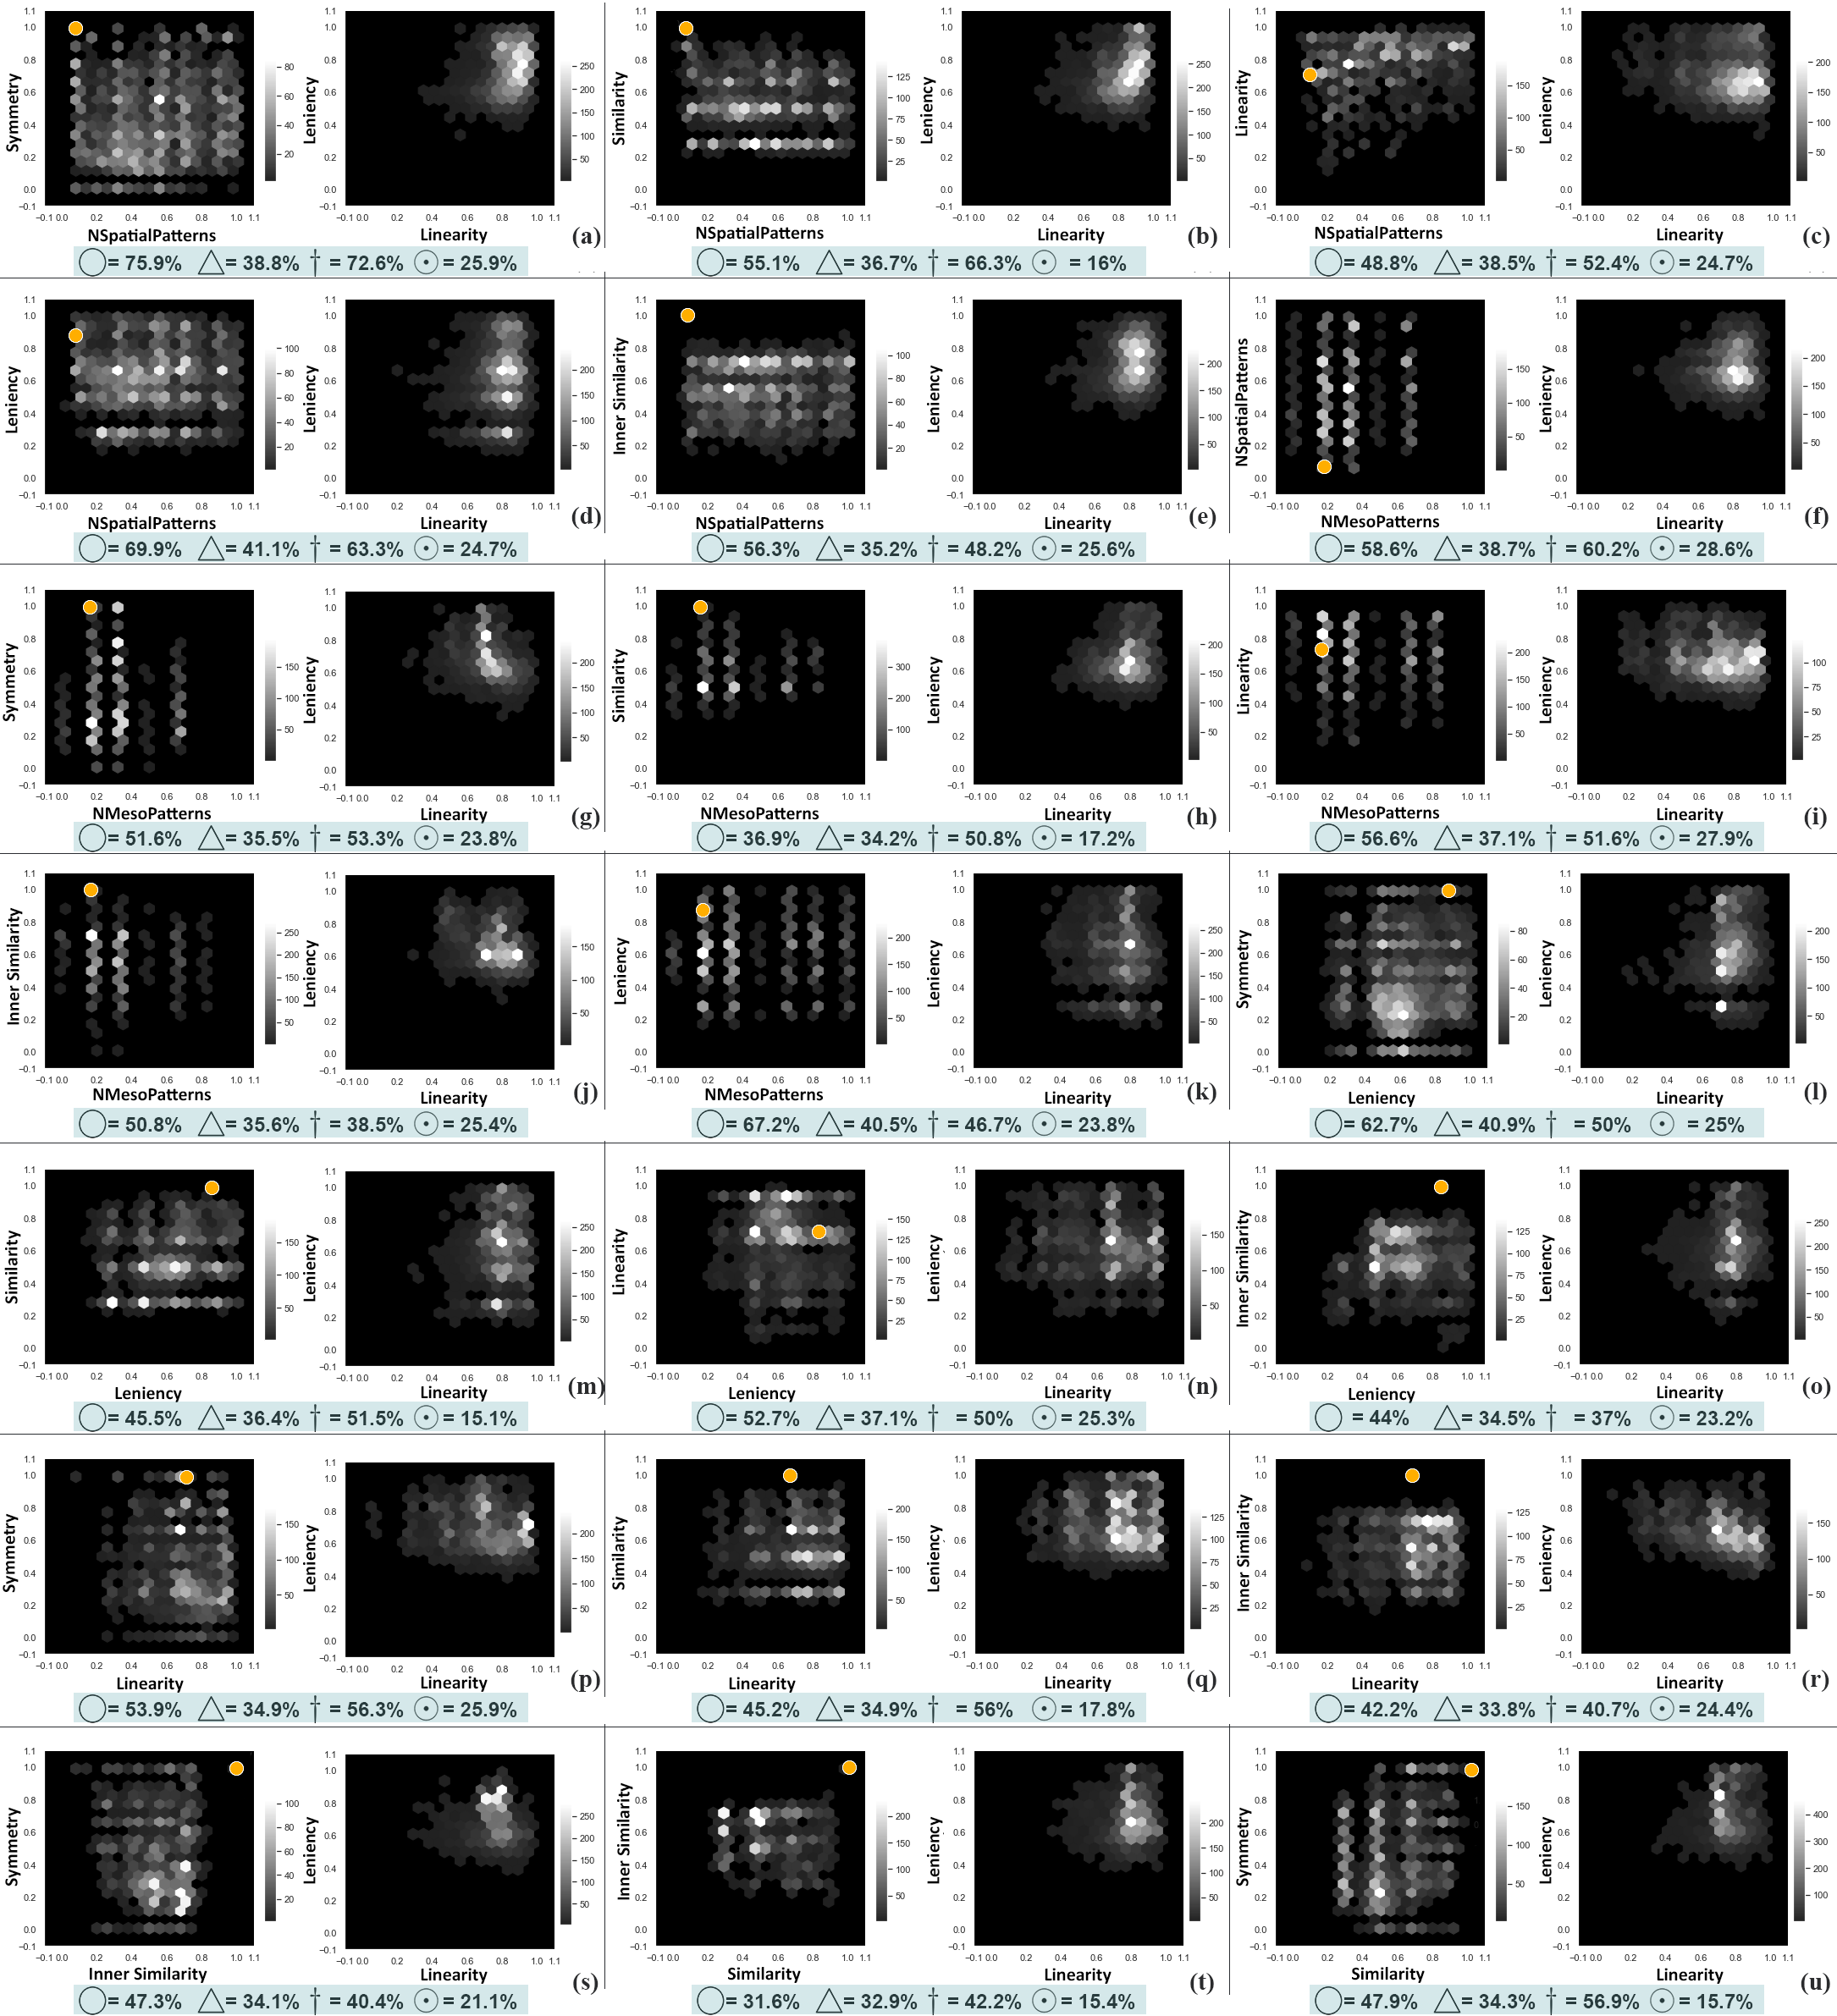
\includegraphics[width=14cm]{figures/figure4.png}}
% \caption{Rooms at generation $2090$ targeting Number of spatial-patterns (X) and Symmetry (Y). Each cell displays (top-right) the fitness of the optimal individual in its related feasible population. }
% \label{figs:patt_sym}
% \end{figure*}



\paragraph{Algorithm}

IC-MAP-Elites is depicted in~\Cref{alg:IC-MAPE}. Cells are first created based on the dimensions selected by the user and proceed to initialize the population based on the user's design, evaluate it and assign each individual to the corresponding cell. Before starting each generation, we check if the dimensions have changed, and if so, recreate the cells and populate them with the previous individuals, and proceed through the evolutionary strategies. We first select uniformly random which cell to choose parents from, and then we select 5 parents through tournament-selection. Offspring are produced through a two-point uniform crossover operation with a 30\% chance of mutation. Offspring are placed in the correct cell and population after calculating their fitness and dimension's information. Finally, cells eliminate the low-performing individuals that over-cap their maximum capacity. Since interbreeding is not allowed, and can only happen indirectly (i.e. the offspring changing population and then used for breeding in consequent generations), the strategies are repeated for each of the populations.

IC MAP-Elites runs for $n$ generations, and once it reaches the specified limit, it broadcasts the found elites. In order to foster the exploration, we first mutate all the individuals from all the populations and cells (while retaining the previous population), and add them into the same pool together with the current edited room without changes. Finally, we evaluate and assign all the individuals to the correct cells, and cells that are over maximum capacity eliminates low-performing individuals. This procedure is repeated until the user decides to stop the algorithm.